% Created by tikzDevice version 0.12.3.1 on 2021-05-25 00:28:46
% !TEX encoding = UTF-8 Unicode
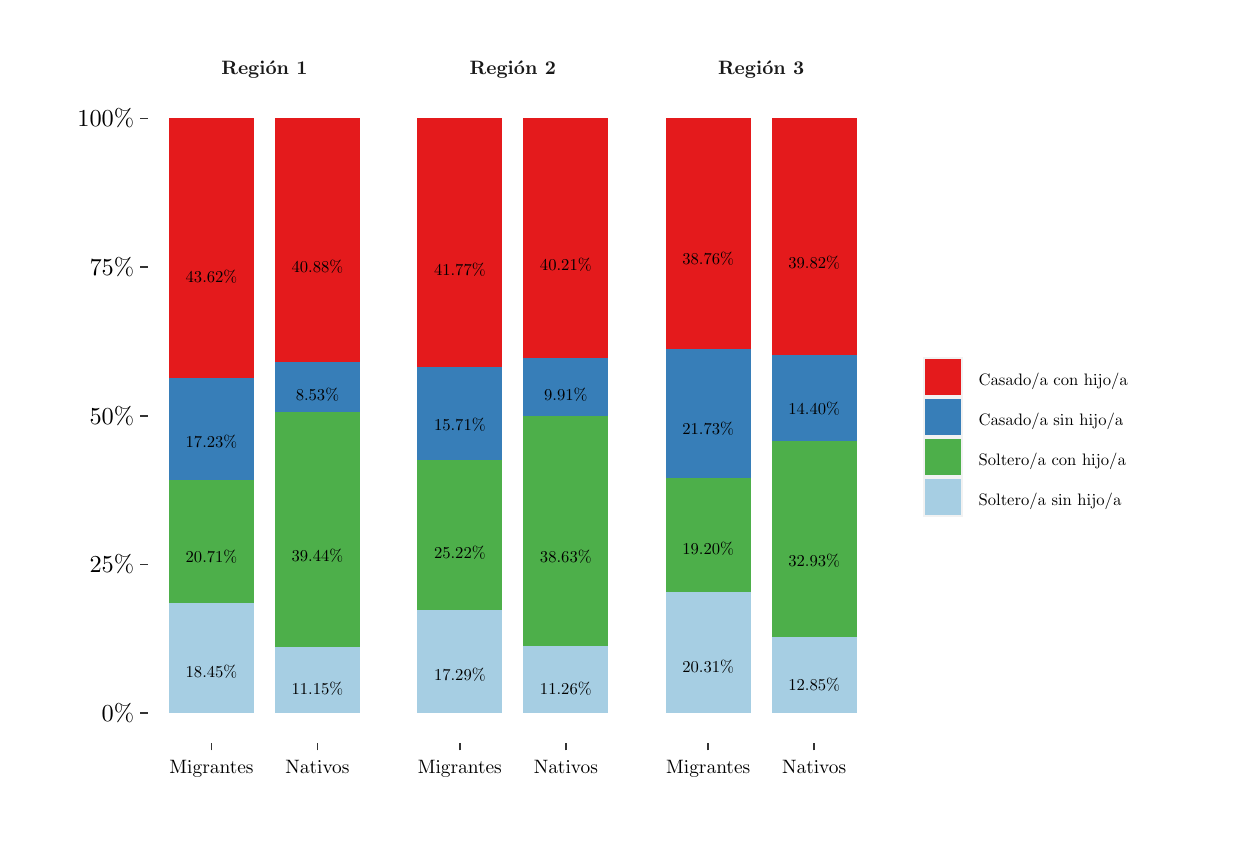
\begin{tikzpicture}[x=1pt,y=1pt]
\definecolor{fillColor}{RGB}{255,255,255}
\path[use as bounding box,fill=fillColor,fill opacity=0.00] (0,0) rectangle (433.62,289.08);
\begin{scope}
\path[clip] (  0.00,  0.00) rectangle (433.62,289.08);
\definecolor{drawColor}{RGB}{255,255,255}
\definecolor{fillColor}{RGB}{255,255,255}

\path[draw=drawColor,line width= 0.6pt,line join=round,line cap=round,fill=fillColor] (  0.00,  0.00) rectangle (433.62,289.08);
\end{scope}
\begin{scope}
\path[clip] ( 43.44, 30.69) rectangle (127.69,267.01);
\definecolor{drawColor}{RGB}{255,255,255}

\path[draw=drawColor,line width= 0.3pt,line join=round] ( 43.44, 68.28) --
	(127.69, 68.28);

\path[draw=drawColor,line width= 0.3pt,line join=round] ( 43.44,121.99) --
	(127.69,121.99);

\path[draw=drawColor,line width= 0.3pt,line join=round] ( 43.44,175.70) --
	(127.69,175.70);

\path[draw=drawColor,line width= 0.3pt,line join=round] ( 43.44,229.41) --
	(127.69,229.41);

\path[draw=drawColor,line width= 0.6pt,line join=round] ( 43.44, 41.43) --
	(127.69, 41.43);

\path[draw=drawColor,line width= 0.6pt,line join=round] ( 43.44, 95.14) --
	(127.69, 95.14);

\path[draw=drawColor,line width= 0.6pt,line join=round] ( 43.44,148.85) --
	(127.69,148.85);

\path[draw=drawColor,line width= 0.6pt,line join=round] ( 43.44,202.56) --
	(127.69,202.56);

\path[draw=drawColor,line width= 0.6pt,line join=round] ( 43.44,256.27) --
	(127.69,256.27);

\path[draw=drawColor,line width= 0.6pt,line join=round] ( 66.42, 30.69) --
	( 66.42,267.01);

\path[draw=drawColor,line width= 0.6pt,line join=round] (104.71, 30.69) --
	(104.71,267.01);
\definecolor{fillColor}{RGB}{228,26,28}

\path[fill=fillColor] ( 51.10,162.56) rectangle ( 81.74,256.27);
\definecolor{fillColor}{RGB}{55,126,184}

\path[fill=fillColor] ( 51.10,125.55) rectangle ( 81.74,162.56);
\definecolor{fillColor}{RGB}{77,175,74}

\path[fill=fillColor] ( 51.10, 81.06) rectangle ( 81.74,125.55);
\definecolor{fillColor}{RGB}{166,206,227}

\path[fill=fillColor] ( 51.10, 41.43) rectangle ( 81.74, 81.06);
\definecolor{fillColor}{RGB}{228,26,28}

\path[fill=fillColor] ( 89.40,168.44) rectangle (120.03,256.27);
\definecolor{fillColor}{RGB}{55,126,184}

\path[fill=fillColor] ( 89.40,150.12) rectangle (120.03,168.44);
\definecolor{fillColor}{RGB}{77,175,74}

\path[fill=fillColor] ( 89.40, 65.38) rectangle (120.03,150.12);
\definecolor{fillColor}{RGB}{166,206,227}

\path[fill=fillColor] ( 89.40, 41.43) rectangle (120.03, 65.38);
\definecolor{drawColor}{RGB}{0,0,0}

\node[text=drawColor,anchor=base,inner sep=0pt, outer sep=0pt, scale=  0.60] at ( 66.42,197.10) {43.62{\%}};

\node[text=drawColor,anchor=base,inner sep=0pt, outer sep=0pt, scale=  0.60] at ( 66.42,137.42) {17.23{\%}};

\node[text=drawColor,anchor=base,inner sep=0pt, outer sep=0pt, scale=  0.60] at ( 66.42, 95.92) {20.71{\%}};

\node[text=drawColor,anchor=base,inner sep=0pt, outer sep=0pt, scale=  0.60] at ( 66.42, 54.34) {18.45{\%}};

\node[text=drawColor,anchor=base,inner sep=0pt, outer sep=0pt, scale=  0.60] at (104.71,200.63) {40.88{\%}};

\node[text=drawColor,anchor=base,inner sep=0pt, outer sep=0pt, scale=  0.60] at (104.71,154.51) {8.53{\%}};

\node[text=drawColor,anchor=base,inner sep=0pt, outer sep=0pt, scale=  0.60] at (104.71, 96.34) {39.44{\%}};

\node[text=drawColor,anchor=base,inner sep=0pt, outer sep=0pt, scale=  0.60] at (104.71, 48.07) {11.15{\%}};
\end{scope}
\begin{scope}
\path[clip] (133.19, 30.69) rectangle (217.43,267.01);
\definecolor{drawColor}{RGB}{255,255,255}

\path[draw=drawColor,line width= 0.3pt,line join=round] (133.19, 68.28) --
	(217.43, 68.28);

\path[draw=drawColor,line width= 0.3pt,line join=round] (133.19,121.99) --
	(217.43,121.99);

\path[draw=drawColor,line width= 0.3pt,line join=round] (133.19,175.70) --
	(217.43,175.70);

\path[draw=drawColor,line width= 0.3pt,line join=round] (133.19,229.41) --
	(217.43,229.41);

\path[draw=drawColor,line width= 0.6pt,line join=round] (133.19, 41.43) --
	(217.43, 41.43);

\path[draw=drawColor,line width= 0.6pt,line join=round] (133.19, 95.14) --
	(217.43, 95.14);

\path[draw=drawColor,line width= 0.6pt,line join=round] (133.19,148.85) --
	(217.43,148.85);

\path[draw=drawColor,line width= 0.6pt,line join=round] (133.19,202.56) --
	(217.43,202.56);

\path[draw=drawColor,line width= 0.6pt,line join=round] (133.19,256.27) --
	(217.43,256.27);

\path[draw=drawColor,line width= 0.6pt,line join=round] (156.16, 30.69) --
	(156.16,267.01);

\path[draw=drawColor,line width= 0.6pt,line join=round] (194.46, 30.69) --
	(194.46,267.01);
\definecolor{fillColor}{RGB}{228,26,28}

\path[fill=fillColor] (140.85,166.53) rectangle (171.48,256.27);
\definecolor{fillColor}{RGB}{55,126,184}

\path[fill=fillColor] (140.85,132.78) rectangle (171.48,166.53);
\definecolor{fillColor}{RGB}{77,175,74}

\path[fill=fillColor] (140.85, 78.58) rectangle (171.48,132.78);
\definecolor{fillColor}{RGB}{166,206,227}

\path[fill=fillColor] (140.85, 41.43) rectangle (171.48, 78.58);
\definecolor{fillColor}{RGB}{228,26,28}

\path[fill=fillColor] (179.14,169.88) rectangle (209.78,256.27);
\definecolor{fillColor}{RGB}{55,126,184}

\path[fill=fillColor] (179.14,148.60) rectangle (209.78,169.88);
\definecolor{fillColor}{RGB}{77,175,74}

\path[fill=fillColor] (179.14, 65.62) rectangle (209.78,148.60);
\definecolor{fillColor}{RGB}{166,206,227}

\path[fill=fillColor] (179.14, 41.43) rectangle (209.78, 65.62);
\definecolor{drawColor}{RGB}{0,0,0}

\node[text=drawColor,anchor=base,inner sep=0pt, outer sep=0pt, scale=  0.60] at (156.16,199.49) {41.77{\%}};

\node[text=drawColor,anchor=base,inner sep=0pt, outer sep=0pt, scale=  0.60] at (156.16,143.34) {15.71{\%}};

\node[text=drawColor,anchor=base,inner sep=0pt, outer sep=0pt, scale=  0.60] at (156.16, 97.32) {25.22{\%}};

\node[text=drawColor,anchor=base,inner sep=0pt, outer sep=0pt, scale=  0.60] at (156.16, 53.35) {17.29{\%}};

\node[text=drawColor,anchor=base,inner sep=0pt, outer sep=0pt, scale=  0.60] at (194.46,201.50) {40.21{\%}};

\node[text=drawColor,anchor=base,inner sep=0pt, outer sep=0pt, scale=  0.60] at (194.46,154.18) {9.91{\%}};

\node[text=drawColor,anchor=base,inner sep=0pt, outer sep=0pt, scale=  0.60] at (194.46, 95.87) {38.63{\%}};

\node[text=drawColor,anchor=base,inner sep=0pt, outer sep=0pt, scale=  0.60] at (194.46, 48.17) {11.26{\%}};
\end{scope}
\begin{scope}
\path[clip] (222.93, 30.69) rectangle (307.18,267.01);
\definecolor{drawColor}{RGB}{255,255,255}

\path[draw=drawColor,line width= 0.3pt,line join=round] (222.93, 68.28) --
	(307.18, 68.28);

\path[draw=drawColor,line width= 0.3pt,line join=round] (222.93,121.99) --
	(307.18,121.99);

\path[draw=drawColor,line width= 0.3pt,line join=round] (222.93,175.70) --
	(307.18,175.70);

\path[draw=drawColor,line width= 0.3pt,line join=round] (222.93,229.41) --
	(307.18,229.41);

\path[draw=drawColor,line width= 0.6pt,line join=round] (222.93, 41.43) --
	(307.18, 41.43);

\path[draw=drawColor,line width= 0.6pt,line join=round] (222.93, 95.14) --
	(307.18, 95.14);

\path[draw=drawColor,line width= 0.6pt,line join=round] (222.93,148.85) --
	(307.18,148.85);

\path[draw=drawColor,line width= 0.6pt,line join=round] (222.93,202.56) --
	(307.18,202.56);

\path[draw=drawColor,line width= 0.6pt,line join=round] (222.93,256.27) --
	(307.18,256.27);

\path[draw=drawColor,line width= 0.6pt,line join=round] (245.91, 30.69) --
	(245.91,267.01);

\path[draw=drawColor,line width= 0.6pt,line join=round] (284.20, 30.69) --
	(284.20,267.01);
\definecolor{fillColor}{RGB}{228,26,28}

\path[fill=fillColor] (230.59,173.00) rectangle (261.23,256.27);
\definecolor{fillColor}{RGB}{55,126,184}

\path[fill=fillColor] (230.59,126.31) rectangle (261.23,173.00);
\definecolor{fillColor}{RGB}{77,175,74}

\path[fill=fillColor] (230.59, 85.07) rectangle (261.23,126.31);
\definecolor{fillColor}{RGB}{166,206,227}

\path[fill=fillColor] (230.59, 41.43) rectangle (261.23, 85.07);
\definecolor{fillColor}{RGB}{228,26,28}

\path[fill=fillColor] (268.89,170.72) rectangle (299.52,256.27);
\definecolor{fillColor}{RGB}{55,126,184}

\path[fill=fillColor] (268.89,139.78) rectangle (299.52,170.72);
\definecolor{fillColor}{RGB}{77,175,74}

\path[fill=fillColor] (268.89, 69.04) rectangle (299.52,139.78);
\definecolor{fillColor}{RGB}{166,206,227}

\path[fill=fillColor] (268.89, 41.43) rectangle (299.52, 69.04);
\definecolor{drawColor}{RGB}{0,0,0}

\node[text=drawColor,anchor=base,inner sep=0pt, outer sep=0pt, scale=  0.60] at (245.91,203.37) {38.76{\%}};

\node[text=drawColor,anchor=base,inner sep=0pt, outer sep=0pt, scale=  0.60] at (245.91,142.05) {21.73{\%}};

\node[text=drawColor,anchor=base,inner sep=0pt, outer sep=0pt, scale=  0.60] at (245.91, 98.63) {19.20{\%}};

\node[text=drawColor,anchor=base,inner sep=0pt, outer sep=0pt, scale=  0.60] at (245.91, 55.94) {20.31{\%}};

\node[text=drawColor,anchor=base,inner sep=0pt, outer sep=0pt, scale=  0.60] at (284.20,202.00) {39.82{\%}};

\node[text=drawColor,anchor=base,inner sep=0pt, outer sep=0pt, scale=  0.60] at (284.20,149.21) {14.40{\%}};

\node[text=drawColor,anchor=base,inner sep=0pt, outer sep=0pt, scale=  0.60] at (284.20, 94.39) {32.93{\%}};

\node[text=drawColor,anchor=base,inner sep=0pt, outer sep=0pt, scale=  0.60] at (284.20, 49.53) {12.85{\%}};
\end{scope}
\begin{scope}
\path[clip] ( 43.44,267.01) rectangle (127.69,283.58);
\definecolor{drawColor}{gray}{0.10}

\node[text=drawColor,anchor=base,inner sep=0pt, outer sep=0pt, scale=  0.70] at ( 85.57,272.26) {\textbf{Región 1}};
\end{scope}
\begin{scope}
\path[clip] (133.19,267.01) rectangle (217.43,283.58);
\definecolor{drawColor}{gray}{0.10}

\node[text=drawColor,anchor=base,inner sep=0pt, outer sep=0pt, scale=  0.70] at (175.31,272.26) {\textbf{Región 2}};
\end{scope}
\begin{scope}
\path[clip] (222.93,267.01) rectangle (307.18,283.58);
\definecolor{drawColor}{gray}{0.10}

\node[text=drawColor,anchor=base,inner sep=0pt, outer sep=0pt, scale=  0.70] at (265.06,272.26) {\textbf{Región 3}};
\end{scope}
\begin{scope}
\path[clip] (  0.00,  0.00) rectangle (433.62,289.08);
\definecolor{drawColor}{gray}{0.20}

\path[draw=drawColor,line width= 0.6pt,line join=round] ( 66.42, 27.94) --
	( 66.42, 30.69);

\path[draw=drawColor,line width= 0.6pt,line join=round] (104.71, 27.94) --
	(104.71, 30.69);
\end{scope}
\begin{scope}
\path[clip] (  0.00,  0.00) rectangle (433.62,289.08);
\definecolor{drawColor}{RGB}{0,0,0}

\node[text=drawColor,anchor=base,inner sep=0pt, outer sep=0pt, scale=  0.70] at ( 66.42, 19.68) {Migrantes};

\node[text=drawColor,anchor=base,inner sep=0pt, outer sep=0pt, scale=  0.70] at (104.71, 19.68) {Nativos};
\end{scope}
\begin{scope}
\path[clip] (  0.00,  0.00) rectangle (433.62,289.08);
\definecolor{drawColor}{gray}{0.20}

\path[draw=drawColor,line width= 0.6pt,line join=round] (156.16, 27.94) --
	(156.16, 30.69);

\path[draw=drawColor,line width= 0.6pt,line join=round] (194.46, 27.94) --
	(194.46, 30.69);
\end{scope}
\begin{scope}
\path[clip] (  0.00,  0.00) rectangle (433.62,289.08);
\definecolor{drawColor}{RGB}{0,0,0}

\node[text=drawColor,anchor=base,inner sep=0pt, outer sep=0pt, scale=  0.70] at (156.16, 19.68) {Migrantes};

\node[text=drawColor,anchor=base,inner sep=0pt, outer sep=0pt, scale=  0.70] at (194.46, 19.68) {Nativos};
\end{scope}
\begin{scope}
\path[clip] (  0.00,  0.00) rectangle (433.62,289.08);
\definecolor{drawColor}{gray}{0.20}

\path[draw=drawColor,line width= 0.6pt,line join=round] (245.91, 27.94) --
	(245.91, 30.69);

\path[draw=drawColor,line width= 0.6pt,line join=round] (284.20, 27.94) --
	(284.20, 30.69);
\end{scope}
\begin{scope}
\path[clip] (  0.00,  0.00) rectangle (433.62,289.08);
\definecolor{drawColor}{RGB}{0,0,0}

\node[text=drawColor,anchor=base,inner sep=0pt, outer sep=0pt, scale=  0.70] at (245.91, 19.68) {Migrantes};

\node[text=drawColor,anchor=base,inner sep=0pt, outer sep=0pt, scale=  0.70] at (284.20, 19.68) {Nativos};
\end{scope}
\begin{scope}
\path[clip] (  0.00,  0.00) rectangle (433.62,289.08);
\definecolor{drawColor}{RGB}{0,0,0}

\node[text=drawColor,anchor=base east,inner sep=0pt, outer sep=0pt, scale=  0.88] at ( 38.49, 38.40) {0{\%}};

\node[text=drawColor,anchor=base east,inner sep=0pt, outer sep=0pt, scale=  0.88] at ( 38.49, 92.11) {25{\%}};

\node[text=drawColor,anchor=base east,inner sep=0pt, outer sep=0pt, scale=  0.88] at ( 38.49,145.82) {50{\%}};

\node[text=drawColor,anchor=base east,inner sep=0pt, outer sep=0pt, scale=  0.88] at ( 38.49,199.53) {75{\%}};

\node[text=drawColor,anchor=base east,inner sep=0pt, outer sep=0pt, scale=  0.88] at ( 38.49,253.24) {100{\%}};
\end{scope}
\begin{scope}
\path[clip] (  0.00,  0.00) rectangle (433.62,289.08);
\definecolor{drawColor}{gray}{0.20}

\path[draw=drawColor,line width= 0.6pt,line join=round] ( 40.69, 41.43) --
	( 43.44, 41.43);

\path[draw=drawColor,line width= 0.6pt,line join=round] ( 40.69, 95.14) --
	( 43.44, 95.14);

\path[draw=drawColor,line width= 0.6pt,line join=round] ( 40.69,148.85) --
	( 43.44,148.85);

\path[draw=drawColor,line width= 0.6pt,line join=round] ( 40.69,202.56) --
	( 43.44,202.56);

\path[draw=drawColor,line width= 0.6pt,line join=round] ( 40.69,256.27) --
	( 43.44,256.27);
\end{scope}
\begin{scope}
\path[clip] (  0.00,  0.00) rectangle (433.62,289.08);
\definecolor{fillColor}{RGB}{255,255,255}

\path[fill=fillColor] (318.18,106.83) rectangle (428.12,190.86);
\end{scope}
\begin{scope}
\path[clip] (  0.00,  0.00) rectangle (433.62,289.08);
\definecolor{fillColor}{gray}{0.95}

\path[fill=fillColor] (323.68,155.69) rectangle (338.13,170.15);
\end{scope}
\begin{scope}
\path[clip] (  0.00,  0.00) rectangle (433.62,289.08);
\definecolor{fillColor}{RGB}{228,26,28}

\path[fill=fillColor] (324.39,156.41) rectangle (337.42,169.44);
\end{scope}
\begin{scope}
\path[clip] (  0.00,  0.00) rectangle (433.62,289.08);
\definecolor{fillColor}{gray}{0.95}

\path[fill=fillColor] (323.68,141.24) rectangle (338.13,155.69);
\end{scope}
\begin{scope}
\path[clip] (  0.00,  0.00) rectangle (433.62,289.08);
\definecolor{fillColor}{RGB}{55,126,184}

\path[fill=fillColor] (324.39,141.95) rectangle (337.42,154.98);
\end{scope}
\begin{scope}
\path[clip] (  0.00,  0.00) rectangle (433.62,289.08);
\definecolor{fillColor}{gray}{0.95}

\path[fill=fillColor] (323.68,126.79) rectangle (338.13,141.24);
\end{scope}
\begin{scope}
\path[clip] (  0.00,  0.00) rectangle (433.62,289.08);
\definecolor{fillColor}{RGB}{77,175,74}

\path[fill=fillColor] (324.39,127.50) rectangle (337.42,140.53);
\end{scope}
\begin{scope}
\path[clip] (  0.00,  0.00) rectangle (433.62,289.08);
\definecolor{fillColor}{gray}{0.95}

\path[fill=fillColor] (323.68,112.33) rectangle (338.13,126.79);
\end{scope}
\begin{scope}
\path[clip] (  0.00,  0.00) rectangle (433.62,289.08);
\definecolor{fillColor}{RGB}{166,206,227}

\path[fill=fillColor] (324.39,113.04) rectangle (337.42,126.07);
\end{scope}
\begin{scope}
\path[clip] (  0.00,  0.00) rectangle (433.62,289.08);
\definecolor{drawColor}{RGB}{0,0,0}

\node[text=drawColor,anchor=base west,inner sep=0pt, outer sep=0pt, scale=  0.60] at (343.63,159.89) {Casado/a con hijo/a};
\end{scope}
\begin{scope}
\path[clip] (  0.00,  0.00) rectangle (433.62,289.08);
\definecolor{drawColor}{RGB}{0,0,0}

\node[text=drawColor,anchor=base west,inner sep=0pt, outer sep=0pt, scale=  0.60] at (343.63,145.44) {Casado/a sin hijo/a};
\end{scope}
\begin{scope}
\path[clip] (  0.00,  0.00) rectangle (433.62,289.08);
\definecolor{drawColor}{RGB}{0,0,0}

\node[text=drawColor,anchor=base west,inner sep=0pt, outer sep=0pt, scale=  0.60] at (343.63,130.98) {Soltero/a con hijo/a};
\end{scope}
\begin{scope}
\path[clip] (  0.00,  0.00) rectangle (433.62,289.08);
\definecolor{drawColor}{RGB}{0,0,0}

\node[text=drawColor,anchor=base west,inner sep=0pt, outer sep=0pt, scale=  0.60] at (343.63,116.53) {Soltero/a sin hijo/a};
\end{scope}
\end{tikzpicture}
